\section{Signaling Protocol}

The signaling protocol plays a fundamental role on our solution, after the web server validates the user access,
it allows the users to directly connect to \ac{KMS} which is placed in a private network and let the server and users negotiate media types and encoding information to use during the conversation.

With respect to the signaling protocol, it could be implemented using \ac{HTTP} messages but they would transport extra information such as \ac{HTTP} headers and would follow a request-response signaling mechanism which would not be the best option, as multiple ice candidates can arrive at any time. Using a \ac{REST} \ac{API} over \ac{HTTP} for signaling and allowing other methods to be called at the same time would lead to open multiple \ac{TCP} connections at the same time.

Instead if we create a \emph{WebSocket} \ac{API} we only need one \ac{TCP} connection and at the same provide bi-directional communications without additional headers. Moreover, using \emph{WebSocket} allows the server to send messages to the client without the client having to request it, which can be slightly faster than using \ac{HTTP}.

Our signaling protocol consists in send and receiving \ac{JSON} formated messages like listing \ref{lst:msgtype} over WebSockets by both the server and the client. 

\begin{minipage}{\linewidth}
\begin{lstlisting}[caption={General structure of our WebSocket messages},label={lst:msgtype},language=json]
{
	"cmd":<cmd>,
	"data":<data>
}
\end{lstlisting}
\end{minipage}

When a user enters in a group conference, after the page is completely loaded it is created a WebSocket that maintains a connection with our web servers. 
Before creating the web socket, we must identify the user and check if he has permissions to participate in the conference. The user identification is done by retrieving the session id from the cookie provided by the user through the \ac{HTTP} headers then we retrieve all the information need from database in order to check if the user has permissions to join the conference room. It's important to save the user identification before the socket is created because after the the handshake performed by the \emph{WebSocket} protocol\cite{rfc6455} the \ac{HTTP} context is lost.

When the connection is established between the server and the client, a \emph{PeerConnection} is created on the client and immediately after an \ac{WebRTC} endpoint on the server specifying a possible set of \ac{ICE} servers to connect.

The user is asked if he wants to share its camera and microphone, share screen or just receive streams from the server. If the user decides to perform a screen share, \emph{adapter.js}\footnote{\url{https://github.com/Temasys/AdapterJS}(accessed March 15, 2015).} may ask to install a plug-in if the browser doesn't support screen sharing.

If the user decides to share either from camera of screen, \emph{getUserMedia} is called with the correspondent constraints in order to obtain a local stream. Use the constraints presented on listing \ref{lst:constraints}. 

\begin{minipage}{\linewidth}
\begin{lstlisting}[caption={Media constraints},label={lst:constraints},language=JavaScript]
var screenShareConstraints = {	
	"video": {
		"mediaSource": "window" || "screen"
	}, 
	"audio": false
};
var cameraMicrophoneConstraints = {
	"audio":true, 
	"video":true 
};
var receiveOnlyConstraints = {
	"offerToReceiveAudio":true,
	"offerToReceiveVideo":true
};
\end{lstlisting}
\end{minipage}

A pop-up is raised in order to ask the user to give permission to share those resources. If the resources are shared successfully the user creates an offer like listing \ref{lst:sig01}, sets a \emph{local session description} to its \emph{PeerConnection} and sends it through WebSockets. If the resources are not shared or the user specified to receive stream only, an offer is created specifying the constraints for receiving only video and audio.

\begin{minipage}{\linewidth}
\begin{lstlisting}[caption={Offer created by client},label={lst:sig01},language=json]
{
	"cmd":"offer",
	"data":{
		"type":"offer",
		"sdp":<sdp>	// this is huge
	}
}
\end{lstlisting}
\end{minipage}

The \emph{local session description} contains the session identifier, codecs, containers, transport protocols and ports used per media type. The \emph{local session description} is useful to conclude if the client is receiving only, which means that \ac{KMS} doesn't need to mix, record and analyze streams coming from the user \ac{WebRTC} endpoint. 

The server receive and processes the offer and sets the \emph{remote session description} to its client associated \ac{WebRTC} endpoint. Then a \emph{local session description} like listing \ref{lst:sig02} is created on the server and sent back to the client, after that the server tries to gather \ac{ICE} candidates.

\begin{minipage}{\linewidth}
\begin{lstlisting}[caption={Answer created by KMS},label={lst:sig02},language=json]
{
	"cmd":"answer",
	"data":{
		"type":"answer",
		"sdp":<sdp>	// this is huge
	}
}
\end{lstlisting}
\end{minipage}

The client receives the server answer, sets the \emph{remote session description} and gets the ice candidates from the \ac{ICE} server. 

Subsequently, after a while both the server and client receive the \ac{ICE} candidates that allow the client to connect directly to \ac{KMS} and vice-versa. The candidates are received at the client which sets them to its \emph{PeerConnection}. The same is done on the server which receives the \ac{ICE} candidates like on listing \ref{lst:sig03} from the client and propagates them to \ac{KMS}.

\begin{minipage}{\linewidth}
\begin{lstlisting}[caption={ICE candidates sent by KMS and client},label={lst:sig03},language=json]
{
	"cmd":"iceCandidate",
	"data":{
		"sdpMLineIndex":0,
		"candidate":"candidate:15 1 TCP 843056127 146.193.224.20 48828 typ srflx raddr 192.168.1.105 rport 48828 tcptype passive",
		"sdpMid":"audio"
	},
}
\end{lstlisting}
\end{minipage}

An \ac{ICE} candidate contains an \ac{IP}, port, used transport protocol and an attribute named \emph{sdpMLineIndex} that is used for mapping to the \emph{remote session description} media type.

In addition both intervenients test the connectivity of each \ac{ICE} candidate. When a connection is established the user and server start to interchange stream data but other \ac{ICE} candidates may arrive with better connections, when that happens the connection changes seamlessly. 

Having the media session established, the server starts to record any received stream and the client creates an \ac{URL} correspondent to the stream location.

\begin{figure}[!htb]
    \centering
    \begin{subfigure}{}
    	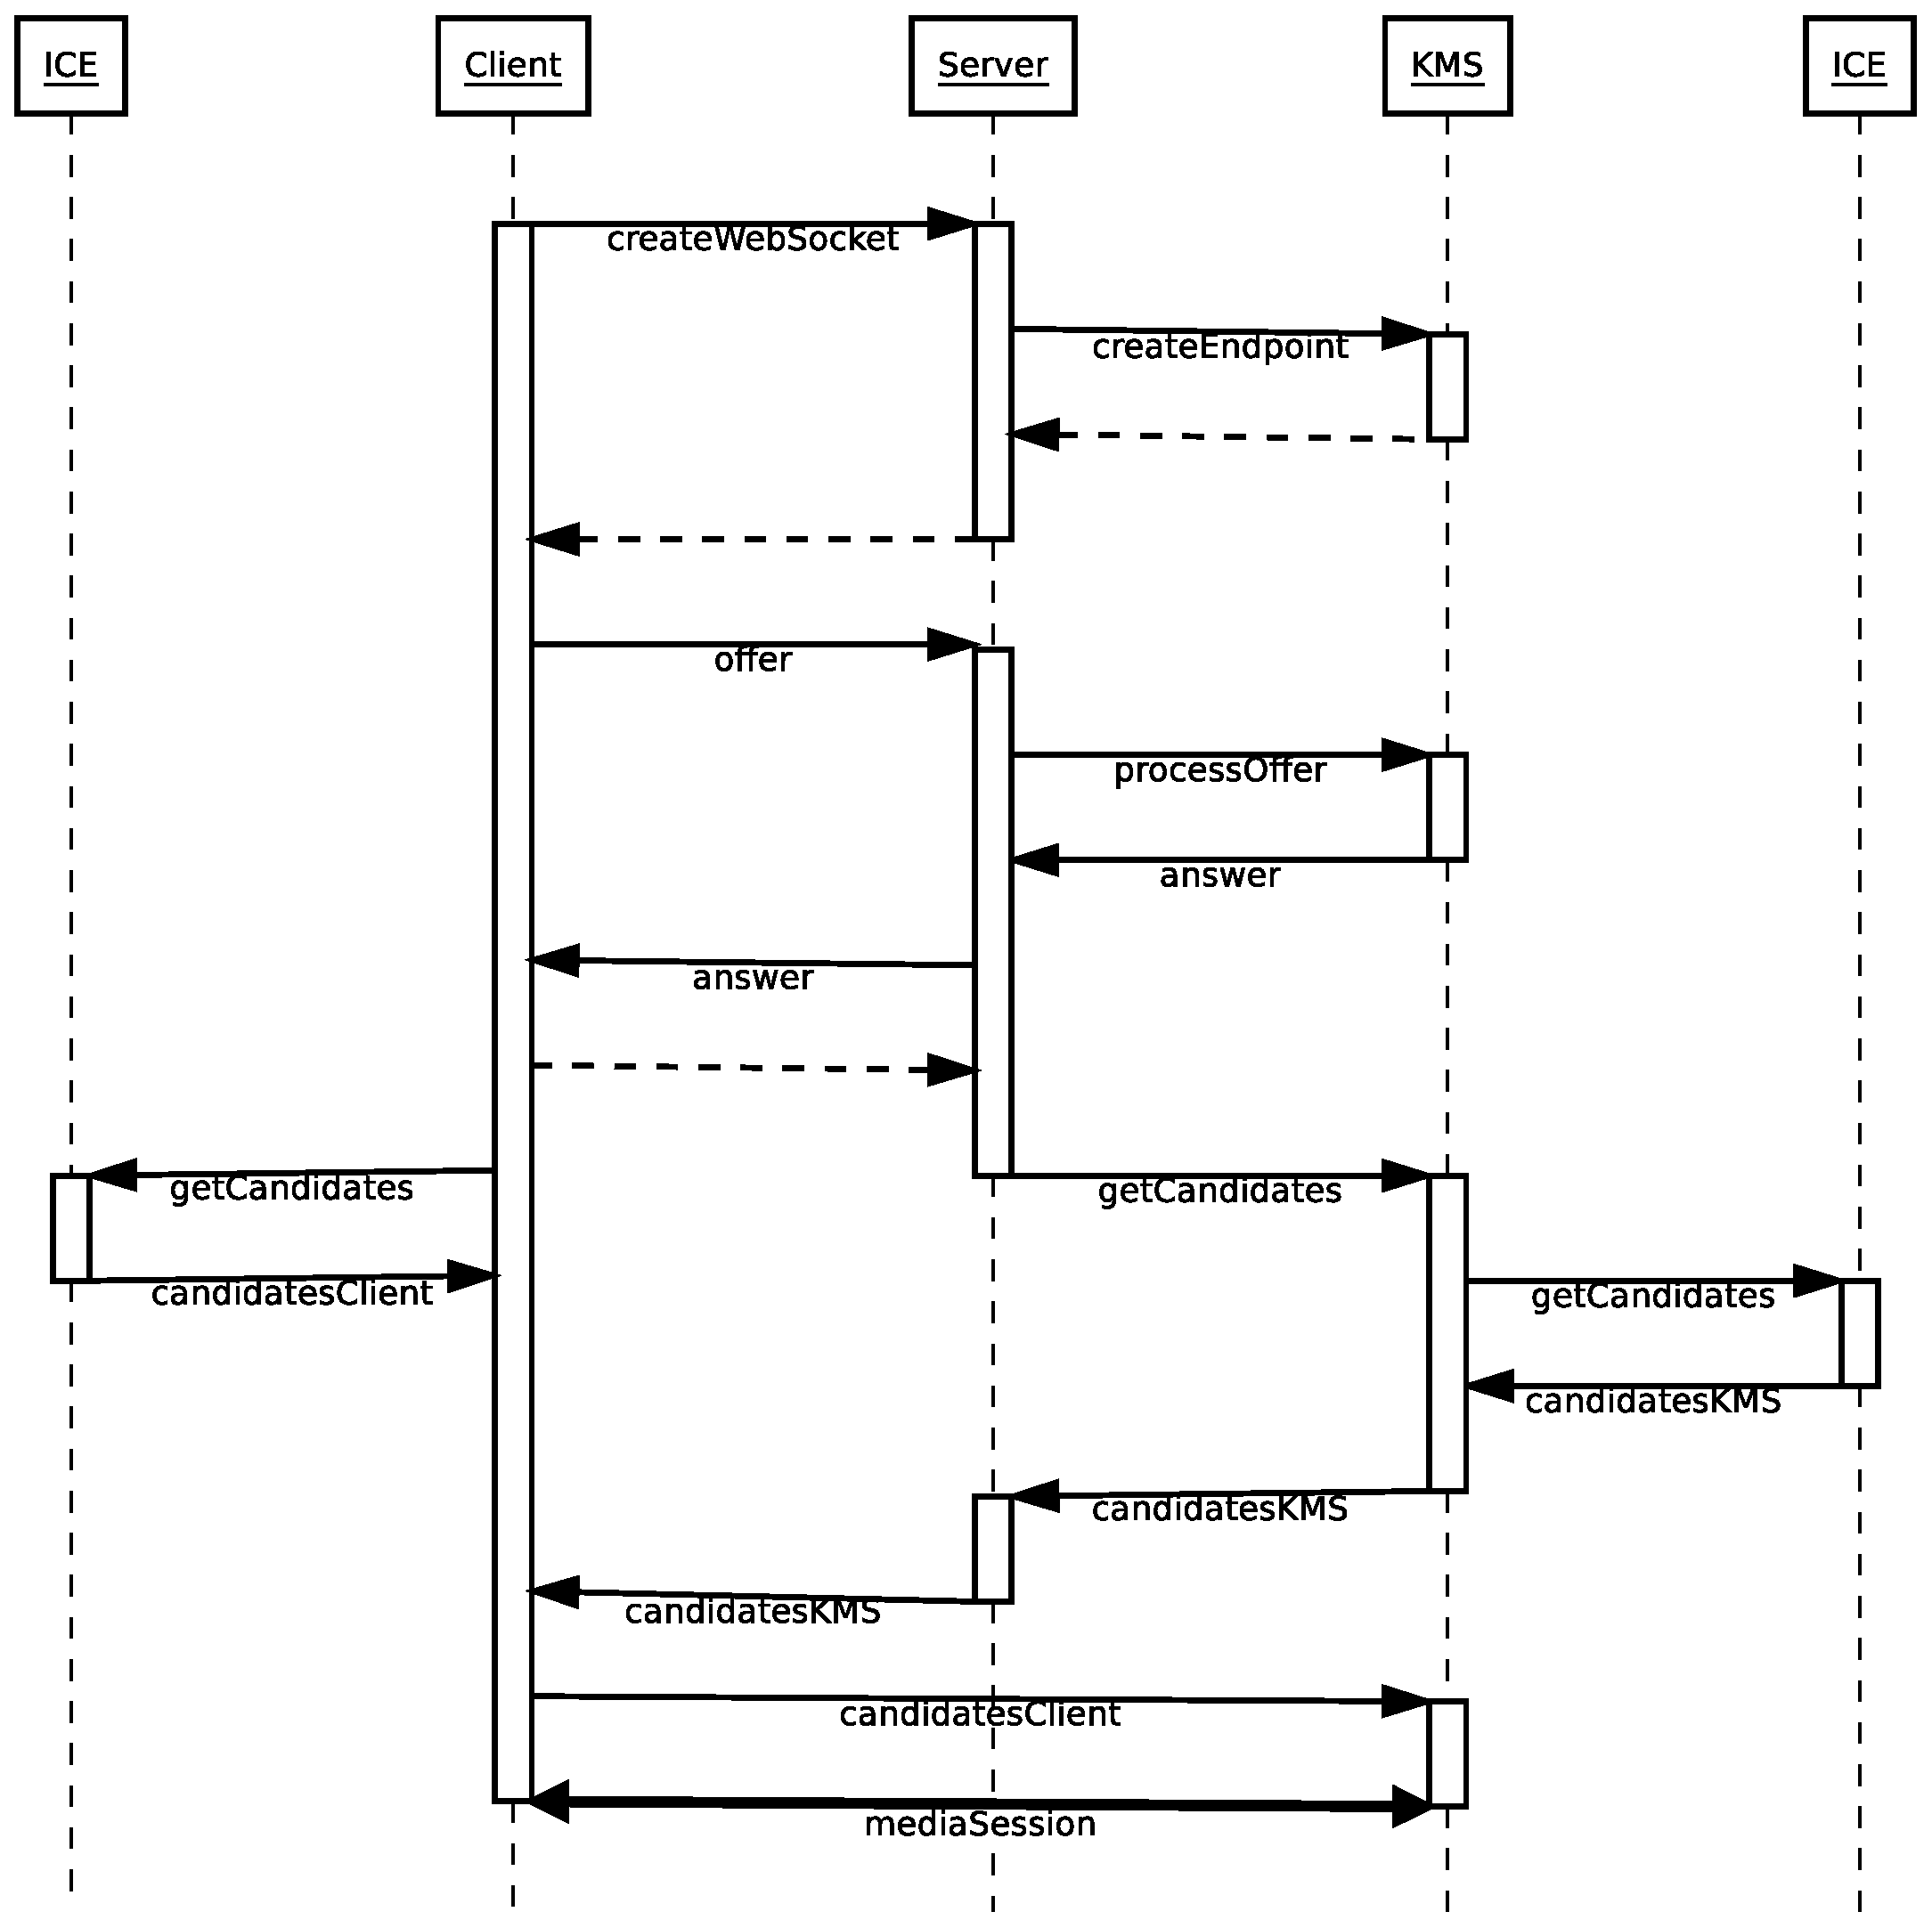
\includegraphics[width=0.9\textwidth]{figures/signaling}
    \end{subfigure}
    \caption{Signaling sequence diagram}
\end{figure} 
